\documentclass[12pt]{scrartcl}
\usepackage[hagavi]{azzam}
\usetikzlibrary{calc,angles}
\renewcommand{\qedsymbol}{$\blacksquare$}

% Geometri Pembuktian Dasar - Solusi
% Pembahasan 12 soal Latihan: 3 Angle Chasing, 3 Kekongruenan,
% 3 Kesebangunan, 3 Segiempat Siklik.
% Penomoran soal sama persis dengan Geometri Pembuktian Dasar_Modul.tex.

\title{Geometri Pembuktian Dasar - Solusi}
\date{13 November 2026}

\begin{document}
\maketitle

\renewcommand*\contentsname{Daftar Isi}
\tableofcontents

\newpage

Pembahasan 12 soal pada berkas Modul. Tiap soal dinyatakan ulang sama
persis dengan nomor yang sama, lalu diikuti solusinya.

\section{Angle Chasing}

\begin{enumerate}

	% Source: OSK SMA 2010 No. 4 (Isian Singkat)
	% Jawaban: 36 derajat
	\item (OSK 2010)
	Diberikan segitiga $ABC$, $AB=AC$. Jika titik $P$ di antara $A$ dan
	$B$ sedemikian rupa sehingga $AP=PC=CB$, maka besarnya sudut $A$
	adalah \dots
\begin{center}
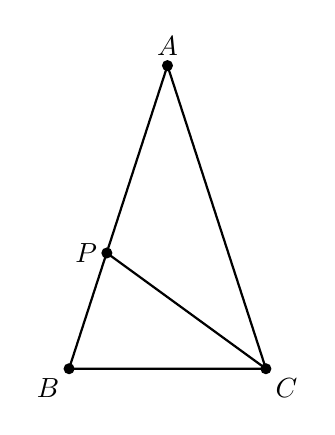
\begin{tikzpicture}[scale=1.0]
    \coordinate (A) at (1.25,3.85);
    \coordinate (B) at (0,0);
    \coordinate (C) at (2.5,0);
    \coordinate (P) at (0.48,1.47);
    \draw[thick] (A) -- (B) -- (C) -- cycle;
    \draw[thick] (P) -- (C);
    \fill (A) circle (2pt);
    \fill (B) circle (2pt);
    \fill (C) circle (2pt);
    \fill (P) circle (2pt);
    \node[above] at (A) {$A$};
    \node[below left] at (B) {$B$};
    \node[below right] at (C) {$C$};
    \node[left] at (P) {$P$};
\end{tikzpicture}
\end{center}
	\begin{proof}[Solusi]
	Tekniknya kejar sudut dengan segitiga sama kaki. Tulis
	$\angle A = \alpha$.
	Segitiga $APC$ sama kaki dengan $AP = PC$, sehingga
	\[ \angle ACP = \angle PAC = \alpha. \]
	Sudut $BPC$ sudut luar segitiga $APC$:
	\[ \angle BPC = \alpha + \alpha = 2\alpha. \]
	Segitiga $PBC$ sama kaki dengan $PC = CB$, sehingga
	\[ \angle PBC = \angle BPC = 2\alpha. \]
	Segitiga $ABC$ sama kaki dengan $AB = AC$, sehingga
	\[ \angle ABC = \angle ACB = 2\alpha. \]
	Jumlah sudut segitiga $ABC$:
	\begin{align*}
	\alpha + 2\alpha + 2\alpha &= 180^\circ, \\
	5\alpha &= 180^\circ, \\
	\alpha &= 36^\circ.
	\end{align*}
	Jadi besarnya sudut $A$ adalah $36^\circ$.
	\end{proof}

	% Source: OSK SMA 2007 No. 16 (Isian Singkat)
	% Jawaban: 135 derajat
	\item (OSK 2007)
	Pada segitiga $PQR$ sama sisi diberikan titik-titik $S$ dan $T$ yang
	terletak berturut-turut pada sisi $QR$ dan $PR$ demikian rupa,
	sehingga $\angle SPR=40^{\circ}$ dan $\angle TQR=35^{\circ}$. Jika
	titik $X$ adalah perpotongan garis-garis $PS$ dan $QT$, maka
	$\angle SXT=\dots$
\begin{center}
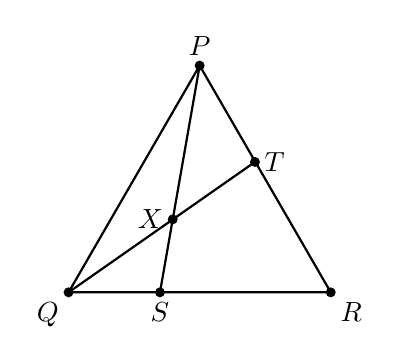
\begin{tikzpicture}[scale=0.9]
    \coordinate (P) at (0,3.2);
    \coordinate (Q) at (-1.85,0);
    \coordinate (R) at (1.85,0);
    \coordinate (S) at (-0.56,0);
    \coordinate (T) at (0.78,1.84);
    \coordinate (X) at (-0.38,1.03);
    \draw[thick] (P) -- (Q) -- (R) -- cycle;
    \draw[thick] (P) -- (S);
    \draw[thick] (Q) -- (T);
    \fill (P) circle (2pt);
    \fill (Q) circle (2pt);
    \fill (R) circle (2pt);
    \fill (S) circle (2pt);
    \fill (T) circle (2pt);
    \fill (X) circle (2pt);
    \node[above] at (P) {$P$};
    \node[below left] at (Q) {$Q$};
    \node[below right] at (R) {$R$};
    \node[below] at (S) {$S$};
    \node[right] at (T) {$T$};
    \node[left] at (X) {$X$};
\end{tikzpicture}
\end{center}
	\begin{proof}[Solusi]
	Tekniknya kejar sudut pada segitiga sama sisi. Semua sudut segitiga
	$PQR$ sama dengan $60^\circ$. Kurangkan sudut yang diketahui:
	\begin{align*}
	\angle SPQ &= 60^\circ - 40^\circ = 20^\circ, \\
	\angle PQT &= 60^\circ - 35^\circ = 25^\circ.
	\end{align*}
	Jumlah sudut segitiga $PQX$:
	\begin{align*}
	\angle PXQ &= 180^\circ - 20^\circ - 25^\circ \\
	&= 135^\circ.
	\end{align*}
	Sudut $SXT$ bertolak belakang dengan sudut $PXQ$, karena $S$
	terletak pada garis $PX$ dan $T$ pada garis $QX$. Jadi
	$\angle SXT = 135^\circ$.
	\end{proof}

	% Source: OSK SMA 2013 No. 8 (Isian Singkat)
	% Jawaban: 80 derajat
	\item (OSK 2013)
	Misalkan $P$ adalah titik interior dalam daerah segitiga $ABC$
	sehingga besar $\angle PAB=10^{\circ}$, $\angle PBA=20^{\circ}$,
	$\angle PCA=30^{\circ}$, $\angle PAC=40^{\circ}$. Besar
	$\angle ABC=\dots$
\begin{center}
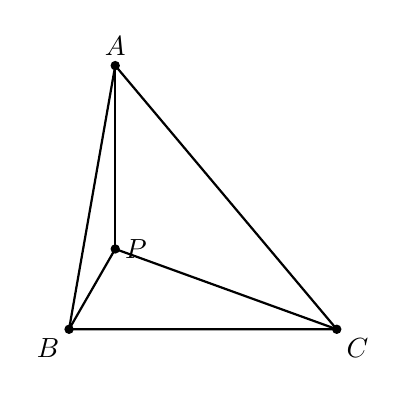
\begin{tikzpicture}[scale=0.85]
    \coordinate (A) at (0.69,3.94);
    \coordinate (B) at (0,0);
    \coordinate (C) at (4,0);
    \coordinate (P) at (0.69,1.20);
    \draw[thick] (A) -- (B) -- (C) -- cycle;
    \draw[thick] (A) -- (P);
    \draw[thick] (B) -- (P);
    \draw[thick] (C) -- (P);
    \fill (A) circle (2pt);
    \fill (B) circle (2pt);
    \fill (C) circle (2pt);
    \fill (P) circle (2pt);
    \node[above] at (A) {$A$};
    \node[below left] at (B) {$B$};
    \node[below right] at (C) {$C$};
    \node[right] at (P) {$P$};
\end{tikzpicture}
\end{center}
	\begin{proof}[Solusi]
	Tekniknya kejar sudut dibantu bentuk trigonometri dari dalil Ceva.
	Tulis $\angle PBC = x$. Besar sudut $A$ segitiga $ABC$:
	\[ \angle BAC = 10^\circ + 40^\circ = 50^\circ, \]
	sehingga besar sudut $C$ segitiga $ABC$:
	$180^\circ - 50^\circ - 20^\circ - x = 110^\circ - x$.
	Sudut $PCB$ sisanya:
	\[ \angle PCB = 110^\circ - x - 30^\circ = 80^\circ - x. \]
	Dalil Ceva trigonometri pada titik $P$ memberi
	\[ \frac{\sin 10^\circ}{\sin 40^\circ} \cdot
	\frac{\sin 30^\circ}{\sin(80^\circ - x)} \cdot
	\frac{\sin x}{\sin 20^\circ} = 1. \]
	Klaim $x = 60^\circ$ memenuhi persamaan ini. Perlu ditunjukkan
	\[ \sin 10^\circ \sin 30^\circ \sin 60^\circ
	= \sin 40^\circ \sin 20^\circ \sin 20^\circ. \]
	Ruas kiri bernilai
	\[ \sin 10^\circ \cdot \frac12 \cdot \frac{\sqrt3}{2}
	= \frac{\sqrt3}{4}\sin 10^\circ. \]
	Ruas kanan dihitung dengan rumus perkalian ke penjumlahan:
	\begin{align*}
	\sin 40^\circ \sin^2 20^\circ
	&= \sin 20^\circ \cdot \frac{\cos 20^\circ - \cos 60^\circ}{2} \\
	&= \frac{2\sin 20^\circ\cos 20^\circ}{4}
	- \frac{\sin 20^\circ}{4} \\
	&= \frac{\sin 40^\circ - \sin 20^\circ}{4} \\
	&= \frac{2\cos 30^\circ\sin 10^\circ}{4} \\
	&= \frac{\sqrt3}{4}\sin 10^\circ.
	\end{align*}
	Kedua ruas sama. Nilai $x$ ini tunggal, karena
	$\dfrac{\sin x}{\sin(80^\circ - x)}$ naik murni untuk
	$0^\circ < x < 80^\circ$: pembilangnya naik, penyebutnya turun
	dan tetap positif. Jadi
	\[ \angle ABC = 20^\circ + 60^\circ = 80^\circ. \]
	\end{proof}

\end{enumerate}

\section{Kekongruenan}

\begin{enumerate}[resume]

	% Source: OSP SMA 2006 No. 17 (Isian Singkat)
	% Jawaban: 180/7 derajat
	\item (OSP 2006)
	Dari titik $O$ ditarik dua sinar garis $l_{1}$ dan $l_{2}$ yang
	membentuk sudut lancip $\alpha$. Titik-titik berbeda $A_{1}, A_{3},
	A_{5}$ terletak pada garis $l_{2}$, sedangkan titik-titik $A_{2},
	A_{4}, A_{6}$ terletak di $l_{1}$. Jika
	$A_{1}A_{2}=A_{2}A_{3}=A_{3}A_{4}=A_{4}O=OA_{5}=A_{5}A_{6}=A_{6}A_{1}$
	maka $\alpha=\dots$
\begin{center}
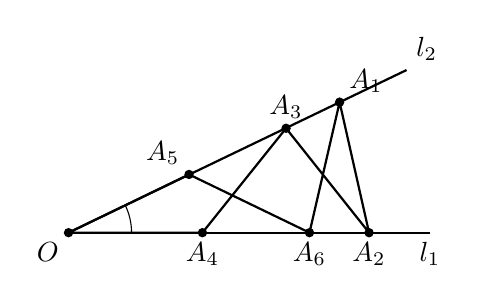
\begin{tikzpicture}[scale=0.85]
    \coordinate (O) at (0,0);
    \coordinate (A4) at (2,0);
    \coordinate (A6) at (3.60,0);
    \coordinate (A2) at (4.49,0);
    \coordinate (A5) at (1.80,0.87);
    \coordinate (A3) at (3.25,1.56);
    \coordinate (A1) at (4.05,1.95);
    \draw[thick] (O) -- (5.4,0);
    \draw[thick] (O) -- (5.05,2.43);
    \draw[thick] (O) -- (A4) -- (A3) -- (A2) -- (A1) -- (A6) -- (A5) -- cycle;
    \pic [draw, angle radius=8mm] {angle = A4--O--A5};
    \fill (O) circle (2pt);
    \fill (A1) circle (2pt);
    \fill (A2) circle (2pt);
    \fill (A3) circle (2pt);
    \fill (A4) circle (2pt);
    \fill (A5) circle (2pt);
    \fill (A6) circle (2pt);
    \node[below left] at (O) {$O$};
    \node[below] at (A4) {$A_4$};
    \node[below] at (A6) {$A_6$};
    \node[below] at (A2) {$A_2$};
    \node[above left] at (A5) {$A_5$};
    \node[above] at (A3) {$A_3$};
    \node[above right] at (A1) {$A_1$};
    \node[below] at (5.4,0) {$l_1$};
    \node[above right] at (5.05,2.43) {$l_2$};
\end{tikzpicture}
\end{center}
	\begin{proof}[Solusi]
	Tekniknya kejar sudut pada rantai segitiga sama kaki. Setiap ruas
	sama panjang, jadi tiap dua ruas berurutan membentuk segitiga sama
	kaki. Kejar dari $O$ melalui dua jalur menuju $A_{1}$.

	Jalur pertama $O \to A_{4} \to A_{3} \to A_{2} \to A_{1}$.
	Segitiga $OA_{4}A_{3}$ sama kaki dengan $OA_{4} = A_{3}A_{4}$:
	\begin{align*}
	\angle OA_{3}A_{4} &= \alpha, \\
	\angle OA_{4}A_{3} &= 180^\circ - 2\alpha.
	\end{align*}
	Sudut $A_{2}A_{4}A_{3}$ berpelurus dengan sudut $OA_{4}A_{3}$:
	\[ \angle A_{2}A_{4}A_{3} = 2\alpha. \]
	Segitiga $A_{4}A_{3}A_{2}$ sama kaki dengan $A_{3}A_{4} = A_{3}A_{2}$:
	\begin{align*}
	\angle A_{4}A_{2}A_{3} &= 2\alpha, \\
	\angle A_{4}A_{3}A_{2} &= 180^\circ - 4\alpha.
	\end{align*}
	Pada titik $A_{3}$, sinar $A_{3}A_{4}$ terletak di antara
	$A_{3}O$ dan $A_{3}A_{2}$, sehingga
	\begin{align*}
	\angle OA_{3}A_{2} &= \alpha + 180^\circ - 4\alpha \\
	&= 180^\circ - 3\alpha.
	\end{align*}
	Sudut $A_{2}A_{3}A_{1}$ berpelurus dengan sudut $OA_{3}A_{2}$
	sepanjang garis $l_{2}$:
	\[ \angle A_{2}A_{3}A_{1} = 3\alpha. \]
	Segitiga $A_{3}A_{2}A_{1}$ sama kaki dengan $A_{2}A_{3} = A_{2}A_{1}$:
	\begin{align*}
	\angle A_{2}A_{1}A_{3} &= 3\alpha, \\
	\angle A_{3}A_{2}A_{1} &= 180^\circ - 6\alpha.
	\end{align*}

	Jalur kedua $O \to A_{5} \to A_{6} \to A_{1}$.
	Segitiga $OA_{5}A_{6}$ sama kaki dengan $OA_{5} = A_{5}A_{6}$:
	\[ \angle OA_{5}A_{6} = 180^\circ - 2\alpha. \]
	Sudut $A_{6}A_{5}A_{1}$ berpelurus dengan sudut $OA_{5}A_{6}$
	sepanjang garis $l_{2}$:
	\[ \angle A_{6}A_{5}A_{1} = 2\alpha. \]
	Segitiga $A_{5}A_{6}A_{1}$ sama kaki dengan $A_{6}A_{5} = A_{6}A_{1}$:
	\[ \angle A_{5}A_{1}A_{6} = 2\alpha. \]

	Pada titik $A_{1}$, kedua ruas $A_{1}A_{2}$ dan $A_{1}A_{6}$ berada
	pada sisi yang sama terhadap garis $l_{2}$. Selisih kedua sudut di
	atas memberi sudut apitnya:
	\[ \angle A_{2}A_{1}A_{6} = 3\alpha - 2\alpha = \alpha. \]
	Segitiga $A_{1}A_{2}A_{6}$ sama kaki dengan $A_{1}A_{2} = A_{1}A_{6}$,
	sehingga sudut alasnya
	\[ \angle A_{1}A_{2}A_{6} = \frac{180^\circ - \alpha}{2}
	= 90^\circ - \frac{\alpha}{2}. \]
	Titik $A_{6}$ terletak pada ruas $OA_{2}$, jadi sudut ini sama
	dengan
	\begin{align*}
	\angle A_{1}A_{2}O &= \angle A_{4}A_{2}A_{3} + \angle A_{3}A_{2}A_{1} \\
	&= 2\alpha + 180^\circ - 6\alpha \\
	&= 180^\circ - 4\alpha.
	\end{align*}
	Samakan kedua nilai:
	\begin{align*}
	180^\circ - 4\alpha &= 90^\circ - \frac{\alpha}{2}, \\
	\frac{7\alpha}{2} &= 90^\circ, \\
	\alpha &= \frac{180^\circ}{7}.
	\end{align*}
	Jadi $\alpha = \dfrac{180^\circ}{7}$.
	\end{proof}

	% Source: OSK SMA 2022 Versi 1 No. 15 (Isian Singkat)
	% Jawaban: 30
	\item (OSK 2022)
	Diberikan segitiga siku-siku sama kaki $ABC$ dengan $BC=AB$.
	Misalkan $L$ titik tengah $BC$ dan $P$ titik pada sisi $AC$ sehingga
	$BP$ tegak lurus $AL$. Jika $CP=10\sqrt{2}$, maka panjang $AB$
	adalah \dots
\begin{center}
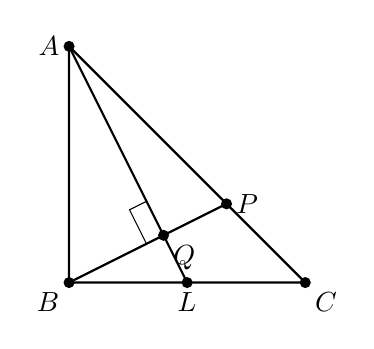
\begin{tikzpicture}[scale=1.0]
    \coordinate (B) at (0,0);
    \coordinate (A) at (0,3);
    \coordinate (C) at (3,0);
    \coordinate (L) at (1.5,0);
    \coordinate (P) at (2,1);
    \coordinate (Q) at (1.2,0.6);
    \draw[thick] (A) -- (B) -- (C) -- cycle;
    \draw[thick] (A) -- (L);
    \draw[thick] (B) -- (P);
    \coordinate (tQa) at ($(Q)!0.18!(A)$);
    \coordinate (tQb) at ($(Q)!0.18!(B)$);
    \draw (tQa) -- ($(tQa)+(tQb)-(Q)$) -- (tQb);
    \fill (A) circle (2pt);
    \fill (B) circle (2pt);
    \fill (C) circle (2pt);
    \fill (L) circle (2pt);
    \fill (P) circle (2pt);
    \fill (Q) circle (2pt);
    \node[left] at (A) {$A$};
    \node[below left] at (B) {$B$};
    \node[below right] at (C) {$C$};
    \node[below] at (L) {$L$};
    \node[right] at (P) {$P$};
    \node[below right] at (Q) {$Q$};
\end{tikzpicture}
\end{center}
	\begin{proof}[Solusi]
	Tekniknya koordinat Kartesius. Sudut siku-siku ada di $B$ sebab
	sisi $AB$ dan $BC$ yang sama panjang. Tulis $AB = BC = s$ dan
	pasang $B = (0,0)$, $A = (0,s)$, $C = (s,0)$. Titik tengah $BC$
	adalah $L = (s/2, 0)$.

	Garis $AL$ berarah $(s/2, -s)$, searah $(1, -2)$. Garis $BP$
	melalui $B$ dan tegak lurus $AL$, jadi berarah $(2, 1)$:
	\[ BP : y = 2x. \]
	Sisi $AC$ menghubungkan $(0,s)$ dan $(s,0)$:
	\[ AC : x + y = s. \]
	Titik $P$ perpotongannya:
	\[ 3x = s, \quad P = \left(\frac{s}{3}, \frac{2s}{3}\right). \]
	Jarak $CP$:
	\begin{align*}
	CP &= \sqrt{\left(\frac{s}{3}\right)^2 + \left(\frac{s}{3}\right)^2} \\
	&= \frac{s\sqrt{2}}{3}.
	\end{align*}
	Diketahui $CP = 10\sqrt{2}$, sehingga $s = 30$. Jadi panjang $AB$
	adalah $30$.
	\end{proof}

	% Source: OSP SMA 2012 No. 19 (Isian Singkat)
	% Jawaban: 90, 60, 30 derajat (sudut C 90, sudut A 60, sudut B 30)
	\item (OSP 2012)
	Diberikan segitiga $ABC$, dengan panjang $AB$ sama dengan dua kali
	panjang $AC$. Misalkan $D$ dan $E$ berturut-turut pada segmen $AB$
	dan $BC$, sehingga $\angle BAE=\angle ACD$. Jika $F=AE \cap CD$ dan
	$CEF$ merupakan segitiga sama sisi, maka besar sudut dari segitiga
	$ABC$ adalah \dots
\begin{center}
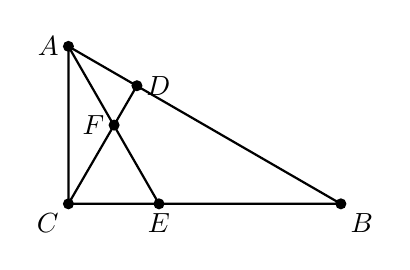
\begin{tikzpicture}[scale=1.0]
    \coordinate (C) at (0,0);
    \coordinate (A) at (0,2);
    \coordinate (B) at (3.46,0);
    \coordinate (E) at (1.15,0);
    \coordinate (F) at (0.58,1.0);
    \coordinate (D) at (0.87,1.5);
    \draw[thick] (A) -- (B) -- (C) -- cycle;
    \draw[thick] (A) -- (E);
    \draw[thick] (C) -- (D);
    \fill (A) circle (2pt);
    \fill (B) circle (2pt);
    \fill (C) circle (2pt);
    \fill (D) circle (2pt);
    \fill (E) circle (2pt);
    \fill (F) circle (2pt);
    \node[left] at (A) {$A$};
    \node[below right] at (B) {$B$};
    \node[below left] at (C) {$C$};
    \node[right] at (D) {$D$};
    \node[below] at (E) {$E$};
    \node[left] at (F) {$F$};
\end{tikzpicture}
\end{center}
	\begin{proof}[Solusi]
	Tekniknya kejar sudut memakai tiga sudut $60^\circ$ dari segitiga
	sama sisi, lalu aturan sinus. Tulis
	$\angle BAE = \angle ACD = \theta$.
	Kedua garis $AE$ dan $CD$ terletak di dalam segitiga.
	Titik potongnya $F$ juga di dalam.

	Pada titik $E$, sudut $FEC = 60^\circ$ dari segitiga sama sisi
	berpelurus dengan sudut $AEB$ sepanjang sisi $BC$:
	\[ \angle AEB = 180^\circ - 60^\circ = 120^\circ. \]
	Jumlah sudut segitiga $ABE$:
	\[ \angle ABE = 180^\circ - \theta - 120^\circ = 60^\circ - \theta. \]
	Karena $E$ terletak pada $BC$, sudut $ABE$ tidak lain adalah sudut $B$ segitiga:
	\[ \angle B = 60^\circ - \theta. \]

	Pada titik $F$, sudut $AFD$ bertolak belakang dengan sudut
	$CFE = 60^\circ$ dari segitiga sama sisi:
	\[ \angle AFD = 60^\circ. \]
	Jumlah sudut segitiga $AFD$, dengan $\angle FAD = \theta$:
	\[ \angle ADF = 180^\circ - \theta - 60^\circ = 120^\circ - \theta. \]
	Jumlah sudut segitiga $ACD$, dengan $\angle ACD = \theta$:
	\begin{align*}
	\angle A &= 180^\circ - \theta - (120^\circ - \theta) \\
	&= 60^\circ.
	\end{align*}

	Sekarang $\angle A = 60^\circ$ dan $\angle B + \angle C = 120^\circ$.
	Aturan sinus pada segitiga $ABC$:
	\[ \frac{AB}{AC} = \frac{\sin C}{\sin B} = 2. \]
	Tulis $C = 120^\circ - B$ dan uraikan:
	\begin{align*}
	\sin(120^\circ - B) &= 2\sin B, \\
	\sin 120^\circ\cos B - \cos 120^\circ\sin B &= 2\sin B, \\
	\frac{\sqrt{3}}{2}\cos B + \frac12\sin B &= 2\sin B, \\
	\frac{\sqrt{3}}{2}\cos B &= \frac32\sin B, \\
	\tan B &= \frac{1}{\sqrt{3}}.
	\end{align*}
	Sudut $B$ lancip, jadi $\angle B = 30^\circ$ dan
	$\angle C = 90^\circ$. Besar ketiga sudutnya:
	$\angle A = 60^\circ$, $\angle B = 30^\circ$,
	$\angle C = 90^\circ$.
	\end{proof}

\end{enumerate}

\section{Kesebangunan}

\begin{enumerate}[resume]

	% Source: OSK SMA 2002 No. 16 (Isian Singkat)
	% Jawaban: 3
	\item (OSK 2002)
	Garis $AB$ dan $CD$ sejajar dan berjarak 4 satuan. Misalkan $AD$
	memotong $BC$ di titik $P$ di antara kedua garis. Jika $AB=4$ dan
	$CD=12$, berapa jauh $P$ dari garis $CD$?
\begin{center}
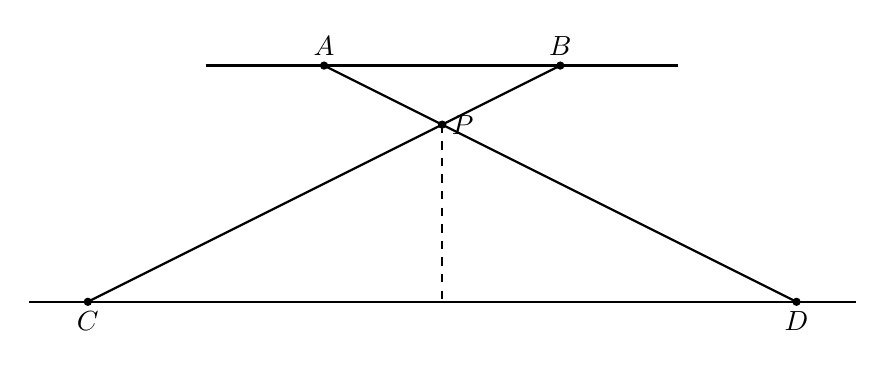
\begin{tikzpicture}[scale=0.75]
    \coordinate (A) at (4,4);
    \coordinate (B) at (8,4);
    \coordinate (C) at (0,0);
    \coordinate (D) at (12,0);
    \coordinate (P) at (6,3);
    \coordinate (H) at (6,0);
    \draw[thick] (2,4) -- (10,4);
    \draw[thick] (-1,0) -- (13,0);
    \draw[thick] (A) -- (D);
    \draw[thick] (B) -- (C);
    \draw[thick,dashed] (P) -- (H);
    \fill (A) circle (2pt);
    \fill (B) circle (2pt);
    \fill (C) circle (2pt);
    \fill (D) circle (2pt);
    \fill (P) circle (2pt);
    \node[above] at (A) {$A$};
    \node[above] at (B) {$B$};
    \node[below] at (C) {$C$};
    \node[below] at (D) {$D$};
    \node[right] at (P) {$P$};
\end{tikzpicture}
\end{center}
	\begin{proof}[Solusi]
	Tekniknya kesebangunan dari garis sejajar. Sudut $PAB$ dan $PDC$
	sama sebagai sudut berseberangan, begitu pula sudut $PBA$ dan
	$PCD$. Jadi
	\[ \triangle PAB \sim \triangle PDC \]
	dengan faktor skala
	\[ \frac{AB}{CD} = \frac{4}{12} = \frac13. \]
	Tinggi kedua segitiga dari $P$ berbanding sama. Tulis $h_{1}$
	jarak $P$ ke garis $AB$ dan $h_{2}$ jarak $P$ ke garis $CD$.
	Titik $P$ di antara kedua garis, sehingga
	\begin{align*}
	\frac{h_{1}}{h_{2}} &= \frac13, \\
	h_{1} + h_{2} &= 4.
	\end{align*}
	Substitusikan $h_{1} = h_{2}/3$:
	\[ \frac{h_{2}}{3} + h_{2} = 4, \quad h_{2} = 3. \]
	Jadi $P$ berjarak $3$ dari garis $CD$.
	\end{proof}

	% Source: OSP SMA 2015 No. 12 (Isian Singkat)
	% Jawaban: 1/2
	\item (OSP 2015)
	Diberikan segitiga $ABC$ dengan $M$ pertengahan $BC$, dan pada sisi
	$AB$ dipilih titik $N$ sehingga $NB=2NA$. Jika
	$\angle CAB=\angle CMN$, maka nilai dari $\frac{AC}{BC}$ adalah
	\dots
\begin{center}
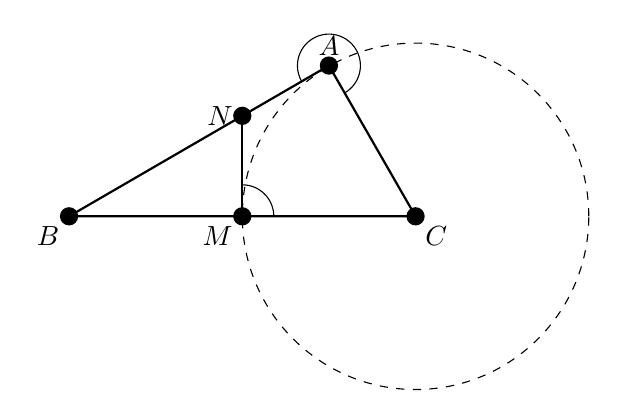
\begin{tikzpicture}[scale=2.2]
    \coordinate (B) at (-1,0);
    \coordinate (C) at (1,0);
    \coordinate (A) at (0.5,0.87);
    \coordinate (M) at (0,0);
    \coordinate (N) at (0,0.58);
    \draw[thick] (A) -- (B) -- (C) -- cycle;
    \draw[thick] (M) -- (N);
    \draw[thin,dashed] (C) circle (1);
    \pic [draw, angle radius=4mm] {angle = C--A--B};
    \pic [draw, angle radius=4mm] {angle = C--M--N};
    \fill (A) circle (1.5pt);
    \fill (B) circle (1.5pt);
    \fill (C) circle (1.5pt);
    \fill (M) circle (1.5pt);
    \fill (N) circle (1.5pt);
    \node[above] at (A) {$A$};
    \node[below left] at (B) {$B$};
    \node[below right] at (C) {$C$};
    \node[below left] at (M) {$M$};
    \node[left] at (N) {$N$};
\end{tikzpicture}
\end{center}
	\begin{proof}[Solusi]
	Tekniknya koordinat Kartesius. Kesamaan sudut memaksa $A$ terletak
	pada lingkaran tertentu. Skalakan $BC = 2$ dan pasang $M = (0,0)$,
	$B = (-1,0)$, $C = (1,0)$, $A = (x,y)$ dengan $y > 0$. Titik $N$
	membagi $AB$ dengan $NB = 2NA$:
	\[ N = A + \frac{B - A}{3}
	= \left(\frac{2x - 1}{3}, \frac{2y}{3}\right). \]

	Sudut $CMN$ di $M$ diapit vektor $MC = (1,0)$ dan
	$MN = ((2x-1)/3, 2y/3)$. Kosinus dan sinusnya:
	\begin{align*}
	\cos\angle CMN &= \frac{2x - 1}{L}, \\
	\sin\angle CMN &= \frac{2y}{L},
	\end{align*}
	dengan $L = \sqrt{(2x-1)^2 + 4y^2} > 0$.

	Sudut $CAB$ di $A$ diapit vektor $B - A = (-1-x, -y)$ dan
	$C - A = (1-x, -y)$. Hasil kali titik dan besar kali silangnya:
	\begin{align*}
	(B - A)\cdot(C - A) &= x^2 + y^2 - 1, \\
	|(B - A)\times(C - A)| &= 2y.
	\end{align*}
	Jadi dengan $b = AC$ dan $c = AB$:
	\begin{align*}
	\cos\angle CAB &= \frac{x^2 + y^2 - 1}{bc}, \\
	\sin\angle CAB &= \frac{2y}{bc}.
	\end{align*}

	Kedua sudut sama dan keduanya di $(0^\circ, 180^\circ)$, sehingga
	tangennya sama:
	\[ \frac{2y}{x^2 + y^2 - 1} = \frac{2y}{2x - 1}. \]
	Dengan $y > 0$ diperoleh $x^2 + y^2 - 1 = 2x - 1$, yaitu
	\[ (x - 1)^2 + y^2 = 1. \]
	(Kasus kedua sudut $90^\circ$ memberi $x^2 + y^2 = 1$ dan
	$x = 1/2$, yang juga memenuhi persamaan ini.)
	Titik $A$ terletak pada lingkaran berpusat $C$ berjari-jari $1$.
	Karena $BC = 2$:
	\[ \frac{AC}{BC} = \frac12. \]
	\end{proof}

	% Source: OSP SMA 2007 No. 18 (Isian Singkat)
	% Jawaban: akar pangkat tiga dari 2
	\item (OSP 2007)
	Diberikan segitiga $ABC$ siku-siku di $A$, titik $D$ pada $AC$ dan
	titik $F$ pada $BC$. Jika $AF \perp BC$ dan $BD=DC=FC=1$, maka
	$AC=\dots$
\begin{center}
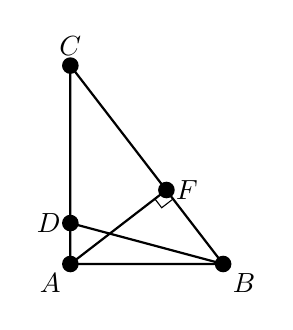
\begin{tikzpicture}[scale=2.0]
    \coordinate (A) at (0,0);
    \coordinate (B) at (0.97,0);
    \coordinate (C) at (0,1.26);
    \coordinate (D) at (0,0.26);
    \coordinate (F) at (0.61,0.47);
    \draw[thick] (A) -- (B) -- (C) -- cycle;
    \draw[thick] (B) -- (D);
    \draw[thick] (A) -- (F);
    \coordinate (tFa) at ($(F)!0.12!(A)$);
    \coordinate (tFb) at ($(F)!0.12!(B)$);
    \draw (tFa) -- ($(tFa)+(tFb)-(F)$) -- (tFb);
    \fill (A) circle (1.5pt);
    \fill (B) circle (1.5pt);
    \fill (C) circle (1.5pt);
    \fill (D) circle (1.5pt);
    \fill (F) circle (1.5pt);
    \node[below left] at (A) {$A$};
    \node[below right] at (B) {$B$};
    \node[above] at (C) {$C$};
    \node[left] at (D) {$D$};
    \node[right] at (F) {$F$};
\end{tikzpicture}
\end{center}
	\begin{proof}[Solusi]
	Tekniknya kesebangunan pada garis tinggi ke sisi miring, lalu
	dalil Pythagoras. Tulis $AC = x$. Titik $D$ pada ruas $AC$ dengan
	$DC = 1$, sehingga $AD = x - 1$.

	Segitiga $AFC$ siku-siku di $F$ dan segitiga $BAC$ siku-siku di
	$A$ berbagi sudut di $C$. Jadi
	\[ \triangle AFC \sim \triangle BAC \]
	dan perbandingan sisi bersesuaiannya:
	\[ \frac{FC}{AC} = \frac{AC}{BC}. \]
	Dengan $FC = 1$ diperoleh $BC = x^2$. Dalil Pythagoras pada
	segitiga $ABC$:
	\[ AB^2 = BC^2 - AC^2 = x^4 - x^2. \]
	Dalil Pythagoras pada segitiga $BAD$ yang siku-siku di $A$,
	dengan $BD = 1$:
	\begin{align*}
	AB^2 + AD^2 &= BD^2, \\
	(x^4 - x^2) + (x - 1)^2 &= 1, \\
	x^4 - 2x &= 0.
	\end{align*}
	Dengan $x > 0$ diperoleh $x^3 = 2$. Jadi
	$AC = \sqrt[3]{2}$.
	\end{proof}

\end{enumerate}

\section{Segiempat Siklik}

\begin{enumerate}[resume]

	% Source: OSK SMA 2005 No. 2 (Pilihan Ganda, disajikan sebagai isian; gambar bintang digambar ulang)
	% Jawaban: 180 derajat
	\item (OSK 2005)
	Pada gambar berikut, $a, b, c, d$ dan $e$ berturut-turut menyatakan
	besar sudut pada titik-titik ujung bintang lima yang terletak pada
	suatu lingkaran. Jumlah $a+b+c+d+e=\dots$

\begin{center}
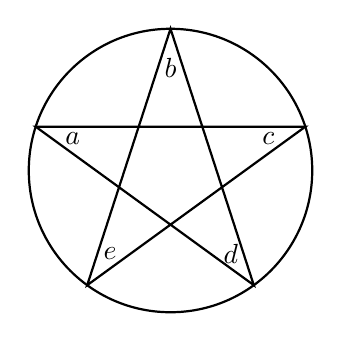
\begin{tikzpicture}[scale=0.9]
    \draw[thick] (0,0) circle (2);
    \coordinate (T) at (90:2);
    \coordinate (L) at (162:2);
    \coordinate (BL) at (234:2);
    \coordinate (BR) at (306:2);
    \coordinate (R) at (18:2);
    \draw[thick] (T) -- (BL) -- (R) -- (L) -- (BR) -- cycle;
    \node at (90:1.45) {$b$};
    \node at (162:1.45) {$a$};
    \node at (18:1.45) {$c$};
    \node at (306:1.45) {$d$};
    \node at (234:1.45) {$e$};
\end{tikzpicture}
\end{center}
	\begin{proof}[Solusi]
	Tekniknya sudut keliling: tiap sudut ujung setengah dari busur
	yang dihadapinya. Namai lima titik ujung menurut urutan
	mengelilingi lingkaran $V_{1}, V_{2}, V_{3}, V_{4}, V_{5}$.
	Sudut di $V_{1}$ diapit tali busur $V_{1}V_{3}$ dan $V_{1}V_{4}$,
	sehingga menghadap busur $V_{3}V_{4}$:
	\[ \text{sudut di } V_{1} = \frac12\,\text{busur } V_{3}V_{4}. \]
	Serupa untuk keempat ujung lain. Kelima busur
	$V_{3}V_{4}$, $V_{4}V_{5}$, $V_{5}V_{1}$, $V_{1}V_{2}$, $V_{2}V_{3}$
	tepat menyusun lingkaran penuh satu kali. Jadi
	\begin{align*}
	a + b + c + d + e &= \frac12 \cdot 360^\circ \\
	&= 180^\circ.
	\end{align*}
	\end{proof}

	% Source: OSP SMA 2025 No. 3 (Isian Singkat; notasi |XY| sumber disederhanakan menjadi XY)
	% Jawaban: 66 derajat
	\item (OSP 2025)
	Diberikan segitiga lancip $ABC$ dengan titik $P$ dan $Q$ pada sisi
	$BC$, titik $R$ pada sisi $AB$ sehingga
	\[ PB=PQ=PR \quad \text{dan} \quad QC=QR. \]
	Diketahui bahwa $ACPR$ merupakan segiempat talibusur. Jika
	$\angle APR=54^\circ$, maka $\angle ABC=\dots$
\begin{center}
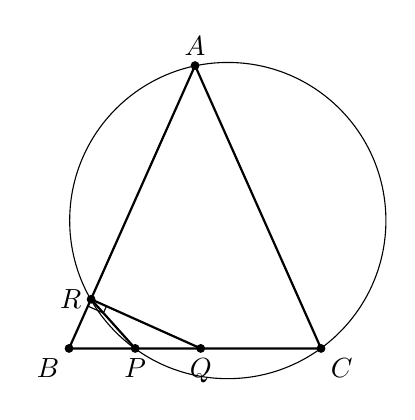
\begin{tikzpicture}[scale=0.8]
    \coordinate (A) at (2,4.49);
    \coordinate (B) at (0,0);
    \coordinate (C) at (4,0);
    \coordinate (P) at (1.05,0);
    \coordinate (Q) at (2.09,0);
    \coordinate (R) at (0.35,0.78);
    \draw[thick] (A) -- (B) -- (C) -- cycle;
    \draw[thick] (P) -- (R);
    \draw[thick] (Q) -- (R);
    \draw[thin] (2.52,2.03) circle (2.51);
    \coordinate (tRb) at ($(R)!0.14!(B)$);
    \coordinate (tRq) at ($(R)!0.14!(Q)$);
    \draw (tRb) -- ($(tRb)+(tRq)-(R)$) -- (tRq);
    \fill (A) circle (2pt);
    \fill (B) circle (2pt);
    \fill (C) circle (2pt);
    \fill (P) circle (2pt);
    \fill (Q) circle (2pt);
    \fill (R) circle (2pt);
    \node[above] at (A) {$A$};
    \node[below left] at (B) {$B$};
    \node[below right] at (C) {$C$};
    \node[below] at (P) {$P$};
    \node[below] at (Q) {$Q$};
    \node[left] at (R) {$R$};
\end{tikzpicture}
\end{center}
	\begin{proof}[Solusi]
	Tekniknya segiempat talibusur dibantu dalil Thales. Tulis
	$\angle ABC = \beta$.

	Titik $P$ dan $Q$ keduanya pada sisi $BC$ dengan $PB = PQ$.
	$Q = B$ mustahil, sebab akibatnya $P = B$ dan sudut $APR$
	degenerasi menjadi $0^\circ$. Jadi urutan pada sisi $BC$ adalah
	$B, P, Q$, dan $P$ titik tengah $BQ$.

	Diketahui $PR = PB = BQ/2$. Titik $R$ berjarak setengah $BQ$
	dari titik tengah $BQ$, jadi $\angle BRQ = 90^\circ$ menurut
	kebalikan dalil Thales. Ruas $RQ$ tegak lurus sisi $AB$.

	Segitiga $BQR$ siku-siku di $R$ dengan sudut $\beta$ di $B$:
	\[ \angle RQB = 90^\circ - \beta. \]
	Sudut $RQC$ berpelurus dengannya sepanjang sisi $BC$:
	\[ \angle RQC = 90^\circ + \beta. \]
	Segitiga $CQR$ sama kaki dengan $QC = QR$, sehingga
	\begin{align*}
	\angle RCB &= \frac{180^\circ - (90^\circ + \beta)}{2} \\
	&= 45^\circ - \frac{\beta}{2}.
	\end{align*}

	Segitiga $BPR$ sama kaki dengan $PB = PR$ dan sudut $\beta$ di
	$B$, sehingga $\angle PRB = \beta$. Sudut $ARP$ berpelurus
	dengannya sepanjang sisi $AB$:
	\[ \angle ARP = 180^\circ - \beta. \]
	Segiempat $ACPR$ talibusur dengan urutan keliling $A, R, P, C$,
	jadi sudut berhadapannya berjumlah $180^\circ$:
	\[ \angle ACP = 180^\circ - \angle ARP = \beta. \]
	Sudut ini sudut $C$ segitiga, jadi $\angle C = \beta$.

	Sudut $APR = 54^\circ$ dan sudut $ACR$ menghadap tali busur $AR$
	yang sama dari sisi yang sama terhadap garis $AB$. Jadi
	\[ \angle ACR = 54^\circ. \]
	Sinar $CR$ membagi sudut $C$ menjadi dua bagian:
	\begin{align*}
	\beta = \angle C &= \angle ACR + \angle RCB \\
	&= 54^\circ + 45^\circ - \frac{\beta}{2}.
	\end{align*}
	Maka $\dfrac{3\beta}{2} = 99^\circ$ dan $\angle ABC = 66^\circ$.
	\end{proof}

	% Source: OSP SMA 2026 No. 1 (Esai)
	% Jawaban: Terbukti
	\item (OSP 2026)
	Misalkan $ABC$ adalah segitiga lancip. Titik $D$ terletak pada garis
	$BC$ sehingga $AD$ tegak lurus $BC$. Misalkan titik $P$ dan $Q$
	berturut-turut merupakan hasil refleksi titik $D$ terhadap garis
	$AB$ dan garis $AC$. Garis $AP$ dan garis $AQ$ memotong lingkaran
	luar $ABC$ berturut-turut di titik $R$ dan $S$ dengan $R\ne A$ dan
	$S\ne A$. Tunjukkan bahwa $AR=AS$.
\begin{center}
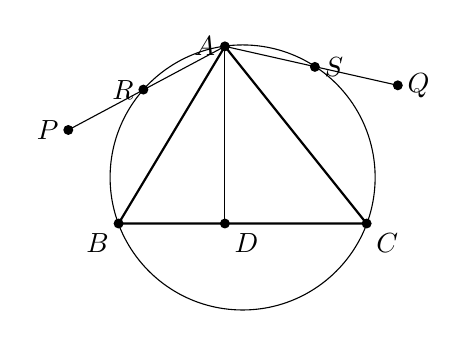
\begin{tikzpicture}[scale=0.9]
    \coordinate (D) at (0,0);
    \coordinate (A) at (0,2.5);
    \coordinate (B) at (-1.5,0);
    \coordinate (C) at (2,0);
    \coordinate (P) at (-2.21,1.32);
    \coordinate (Q) at (2.44,1.95);
    \coordinate (R) at (-1.15,1.89);
    \coordinate (S) at (1.27,2.21);
    \draw[thick] (A) -- (B) -- (C) -- cycle;
    \draw[thin] (A) -- (D);
    \draw[thin] (0.25,0.65) circle (1.87);
    \draw[thin] (A) -- (P);
    \draw[thin] (A) -- (Q);
    \fill (A) circle (2pt);
    \fill (B) circle (2pt);
    \fill (C) circle (2pt);
    \fill (D) circle (2pt);
    \fill (P) circle (2pt);
    \fill (Q) circle (2pt);
    \fill (R) circle (2pt);
    \fill (S) circle (2pt);
    \node[left] at (A) {$A$};
    \node[below left] at (B) {$B$};
    \node[below right] at (C) {$C$};
    \node[below right] at (D) {$D$};
    \node[left] at (P) {$P$};
    \node[right] at (Q) {$Q$};
    \node[left] at (R) {$R$};
    \node[right] at (S) {$S$};
\end{tikzpicture}
\end{center}
	\begin{proof}[Solusi]
	Tekniknya koordinat Kartesius pada lingkaran luar. Segitiga
	lancip menempatkan $D$ di dalam ruas $BC$. Pasang $D = (0,0)$,
	$A = (0,t)$, $B = (-b,0)$, $C = (c,0)$ dengan $b, c, t > 0$.

	Lingkaran luar $ABC$ berpusat di $O = (h,k)$ dengan $h$
	titik tengah $BC$:
	\[ h = \frac{c - b}{2}. \]
	Samakan kuadrat jarak $O$ ke $B$ dan ke $A$:
	\begin{align*}
	(h + b)^2 + k^2 &= h^2 + (k - t)^2, \\
	2hb + b^2 &= -2kt + t^2.
	\end{align*}
	Dengan $2hb = b(c - b)$ diperoleh
	\[ k = \frac{t^2 - bc}{2t}. \]

	Garis $AP$ pencerminan garis $AD$ terhadap garis $AB$.
	Vektor satuan sepanjang $AB$ adalah $u = (b,t)/\sqrt{S}$ dengan
	$S = t^2 + b^2$. Cerminkan arah $AD$, yaitu $(0,1)$:
	\begin{align*}
	d &= 2((0,1)\cdot u)u - (0,1) \\
	&= \frac{2t}{S}(b,t) - (0,1) \\
	&= \frac{1}{S}(2bt, t^2 - b^2).
	\end{align*}
	Garis $AP$ berarah $d' = (2bt, t^2 - b^2)$ dengan
	$|d'|^2 = (t^2 + b^2)^2 = S^2$.
	Tulis titiknya $X(\lambda) = A + \lambda d'$. Potongannya dengan
	lingkaran memenuhi $|X(\lambda) - O|^2 = R^2$, persamaan kuadrat
	dengan akar $\lambda = 0$ di $A$. Akar lainnya:
	\[ \lambda_R = -\frac{2d'\cdot(A - O)}{|d'|^2}. \]
	Vektor $A - O = (-h, t - k)$ dengan
	$t - k = \dfrac{t^2 + bc}{2t}$. Hasil kali titiknya:
	\begin{align*}
	d'\cdot(A - O) &= -2bth + (t^2 - b^2)(t - k) \\
	&= \frac{S(t^2 - bc)}{2t}.
	\end{align*}
	Jadi
	\[ \lambda_R = -\frac{t^2 - bc}{tS}, \quad
	AR = |\lambda_R|\cdot|d'| = \frac{t^2 - bc}{t}. \]
	Nilai $t^2 - bc > 0$ sebab sudut $A$ lancip.
	Cerminan terhadap sumbu $y$ menukar peran $b$ dan $c$, sehingga perhitungan
	yang sama untuk garis $AQ$ memberi
	\[ AS = \frac{t^2 - bc}{t}. \]
	Kedua panjang sama. Terbukti $AR = AS$.
	\end{proof}

\end{enumerate}

\end{document}
